\documentclass[11pt]{beamer}
\usetheme{Madrid}
\usefonttheme{serif}

\usepackage[utf8]{inputenc}
\usepackage[english]{babel}
\usepackage[T1]{fontenc}

\usepackage{amsmath}
\usepackage{amsfonts}
\usepackage{amssymb}
\usepackage{graphicx}

% Add adjustbox for better table scaling
\usepackage{adjustbox}

\setbeamertemplate{caption}[numbered]
\setbeamertemplate{navigation symbols}{}

% Author / Title Info
\title{Offline 2D-to-3D Reconstruction System for ARM-Based Mobile Devices}

\author{
Goureesh Chandra (TVE22CS069) \\ 
Ivin Mathew Kurian (TVE22CS075) \\ 
Muhammed Farhan (TVE22CS094) \\ 
Rethin Francis (LTV22CS149) \\[6pt]
\textbf{Advisor: Prof. Divya S K}
}

\institute{
College of Engineering, Trivandrum \\ 
Dept. of Computer Science \& Engineering
}

\date{\today}

% ---------------------------------------------------------
\begin{document}

% Title
\begin{frame}
\titlepage
\end{frame}



% Table of Contents
\begin{frame}{Contents}
  \tableofcontents
\end{frame}

% --------------------------------------
\section{Introduction}
\begin{frame}{Introduction}
\begin{itemize}
\item Three-dimensional (3D) reconstruction from two-dimensional (2D) images is an important problem in computer vision.
\item Most existing 3D reconstruction systems depend on cloud servers or high-end computing hardware.
\item Such solutions are not suitable for mobile, offline, and resource-constrained environments.
\item This project focuses on enabling efficient and fully offline 2D-to-3D reconstruction on ARM-based mobile devices.
\end{itemize}
\end{frame}

% --------------------------------------
\section{Objective}
\begin{frame}{Objective}
The objective of this project is to develop a fully offline 2D-to-3D reconstruction system for ARM-based mobile devices.

\medskip
\begin{itemize}
\item \textbf{Lightweight Depth Estimation Module} -- estimate dense depth maps from single or multiple images using an on-device neural network.
\item \textbf{Geometric Processing Pipeline} -- compute camera poses and fuse multiple depth maps into a unified 3D representation.
\item \textbf{On-Device Mesh Generation and Visualization} -- extract and render a 3D surface mesh in real time without cloud dependency.
\end{itemize}
\end{frame}

% --------------------------------------
\section{Problem Statement}

\begin{frame}{Problem Statement}
Most existing 2D-to-3D reconstruction systems rely on cloud servers or high-performance computing hardware to achieve acceptable accuracy and speed.

\medskip
Such approaches:
\begin{itemize}
\item Require continuous internet connectivity and powerful GPUs.
\item Are unsuitable for real-time use on resource-constrained mobile devices.
\item Raise privacy concerns due to off-device data processing.
\item Limit accessibility and portability for everyday users.
\end{itemize}

\medskip
Hence, there is a need for a \textbf{fully offline, efficient, and mobile-optimized} 2D-to-3D reconstruction system that can operate directly on ARM-based devices.
\end{frame}

% --------------------------------------

\section{Literature Review}

\begin{frame}[allowframebreaks]{Literature Review}
\small

\begin{adjustbox}{max width=\textwidth}
\begin{tabular}{|p{0.8cm}|p{3.5cm}|p{2.5cm}|p{3cm}|p{1.5cm}|p{4cm}|}
\hline
\textbf{Sl. No} &
\textbf{Publication} &
\textbf{Journal/Conf.} &
\textbf{Author(s)} &
\textbf{Year} &
\textbf{Observation} \\
\hline

1 & TripoSR: Fast 3D Object Reconstruction from a Single Image &
arXiv &
D. Tochilkin et al. &
2024 &
Transformer-based single-image 3D reconstruction producing high quality meshes but requiring powerful GPUs. \\
\hline

2 & Mobile3DRecon: Real-time Monocular 3D Reconstruction on a Mobile Phone &
IEEE TVCG &
X. Yang et al. &
2020 &
Designed for smartphones and supports real-time processing but lacks modern deep learning models. \\
\hline

3 & METER: A Mobile Vision Transformer Architecture for Monocular Depth Estimation &
IEEE Journal &
L. Papa et al. &
2024 &
Vision transformer optimized for embedded devices enabling efficient depth estimation. \\
\hline

4 & LiteDepth: Fast and Accurate Depth Estimation on Mobile Devices &
ECCV &
Z. Li et al. &
2022 &
Ultra-lightweight CNN architecture designed for mobile depth estimation. \\
\hline

\end{tabular}
\end{adjustbox}

\end{frame}

\begin{frame}[allowframebreaks]{Literature Review}
\small

\begin{adjustbox}{max width=\textwidth}
\begin{tabular}{|p{0.8cm}|p{3.5cm}|p{2.5cm}|p{3cm}|p{1.5cm}|p{4cm}|}
\hline
\textbf{Sl. No} &
\textbf{Publication} &
\textbf{Journal/Conf.} &
\textbf{Author(s)} &
\textbf{Year} &
\textbf{Observation} \\
\hline

5 & Large-Scale 3D Reconstruction from Multi-View Imagery: A Comprehensive Review &
Remote Sensing &
H. Luo et al. &
2024 &
Survey of multi-view stereo, SfM and NeRF based reconstruction techniques. \\
\hline

6 & 3D Reconstruction Using Deep Learning: A Survey &
IEEE TPAMI &
A. Smith et al. &
2023 &
Overview of deep learning approaches for 3D reconstruction and their computational challenges. \\
\hline

7 & Real-Time 3D Object Reconstruction and Distance Estimation from 2D Images &
IJCV &
B. Johnson et al. &
2022 &
Pipeline using computer vision tools like OpenCV for real-time object reconstruction. \\
\hline

8 & ZoeDepth: Zero-shot Transfer by Combining Relative and Metric Depth &
arXiv &
C. Lee et al. &
2023 &
Zero-shot depth estimation model with strong cross-dataset generalization. \\
\hline

\end{tabular}
\end{adjustbox}

\end{frame}


% --------------------------------------
\section{Proposed Solution Methodology}

\begin{frame}{Proposed Solution Methodology}
The proposed system follows a structured pipeline to achieve fully offline 2D-to-3D reconstruction on ARM-based mobile devices.

\medskip
\begin{itemize}
\item \textbf{Image Acquisition} -- Capture one or multiple 2D images using the mobile device camera.
\item \textbf{Monocular Depth Estimation} -- Generate dense depth maps using a lightweight on-device neural network.
\item \textbf{Camera Pose Estimation} -- Estimate camera positions and orientations through feature matching between frames.
\item \textbf{Depth Fusion} -- Integrate multiple depth maps into a unified 3D representation using efficient geometric techniques.
\item \textbf{Mesh Generation and Visualization} -- Extract a surface mesh and render it in real time on the mobile device.
\end{itemize}
\end{frame}

% ------------------------------------------------------
\section{Algorithm}

\begin{frame}{Algorithm 1: Offline 2D-to-3D Reconstruction}
\textbf{Goal:} Generate a 3D surface model from 2D images entirely on-device.

\medskip
\textbf{Steps:}
\begin{enumerate}
\item \textbf{Initialization:}
\begin{itemize}
\item Load lightweight depth estimation model parameters.
\item Initialize feature extractor and geometric fusion modules.
\end{itemize}

\item \textbf{Processing Loop:}
\begin{enumerate}
\item Capture one or more RGB images from the mobile camera.
\item Estimate dense depth maps using the on-device neural network.
\item Extract and match visual features between frames.
\item Estimate camera poses using feature correspondences.
\item Fuse multiple depth maps into a unified 3D representation.
\end{enumerate}

\item \textbf{Output:}
\begin{itemize}
\item Generate and display a 3D surface mesh in real time.
\end{itemize}
\end{enumerate}
\end{frame}

% ------------------------------------------------------
\begin{frame}{Algorithm 2: Depth Fusion and Mesh Generation}
\textbf{Goal:} Construct a consistent 3D surface from multiple depth maps.

\medskip
\textbf{Steps:}
\begin{enumerate}
\item Align depth maps using estimated camera poses.
\item Integrate depth information into a common coordinate frame.
\item Filter noise and inconsistencies in fused depth data.
\item Extract surface mesh using geometric reconstruction techniques.
\item Optimize mesh for efficient rendering on mobile devices.
\end{enumerate}

\medskip
\textbf{Output:} Optimized 3D surface mesh for real-time visualization.
\end{frame}

% --------------------------------------
\section{Resource Allocation}

\begin{frame}{Resource Allocation}
\textbf{1. Data Resources}
\begin{itemize}
\item 2D image datasets (indoor and outdoor scenes).
\item Mobile camera images captured under real-world conditions.
\item Preprocessing tools: OpenCV, NumPy.
\end{itemize}

\medskip
\textbf{2. Computational Resources}
\begin{itemize}
\item ARM-based mobile device for deployment.
\item Development system with GPU support for model training.
\item Frameworks: PyTorch, TensorFlow Lite.
\end{itemize}
\end{frame}

\begin{frame}{Resource Allocation (cont.)}
\textbf{3. Methodology-Specific Tools}
\begin{itemize}
\item Lightweight depth estimation models.
\item Feature matching and pose estimation algorithms.
\item 3D processing libraries: Open3D, OpenGL.
\end{itemize}

\medskip
\textbf{4. Human Resources \& Timeline}
\begin{itemize}
\item Team: 4 student developers, 1 faculty advisor.
\item Model optimization: 4 weeks.
\item System integration and testing: 6 weeks.
\item Evaluation and documentation: 3 weeks.
\end{itemize}
\end{frame}

%-----------------------------
\section{Model Comparison}

\begin{frame}{Comparison with Existing Models}
\centering
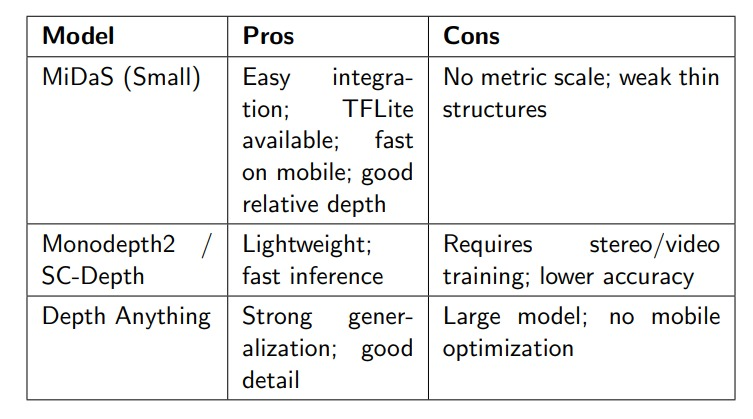
\includegraphics[width=\textwidth,height=0.85\textheight,keepaspectratio]{png1.jpeg}
\end{frame}

%---------------------------------
\begin{frame}{Comparison with Existing Models}
\centering
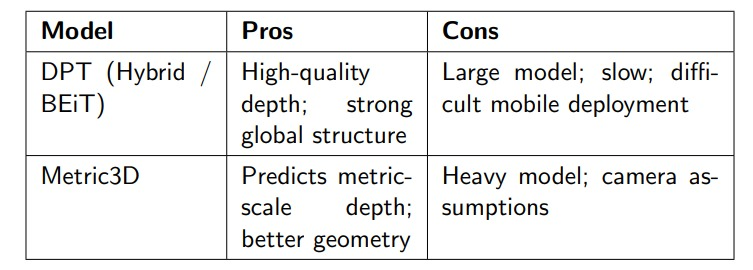
\includegraphics[width=\textwidth,height=0.85\textheight,keepaspectratio]{png2.jpeg}
\end{frame}

%-----------------------------------
\begin{frame}{Comparison with Existing Models}
\centering
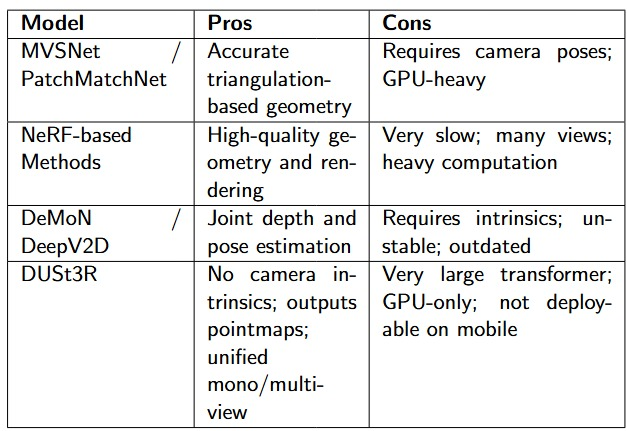
\includegraphics[width=\textwidth,height=0.85\textheight,keepaspectratio]{png3.jpeg}
\end{frame}

\section{Novelty of the Idea}

\begin{frame}{Novelty of the Proposed System}
\begin{itemize}
\item Fully offline 2D-to-3D reconstruction system designed for mobile devices.
\item Uses lightweight depth estimation models optimized for ARM processors.
\item Combines ARCore spatial tracking with neural depth estimation.
\item Performs point cloud generation and visualization directly on the mobile device.
\item Avoids heavy GPU-based rendering by using a CPU-based rendering pipeline in Flutter.
\end{itemize}
\end{frame}

\section{Modules of the Project}

\begin{frame}{Modules of the Proposed System}
\begin{itemize}
\item \textbf{AR Capture Module}
\begin{itemize}
\item Captures RGB images and camera pose using ARCore.
\item Uses virtual anchors to maintain spatial reference.
\end{itemize}

\item \textbf{Depth Estimation Module}
\begin{itemize}
\item Uses MiDaS model converted to TensorFlow Lite.
\item Generates dense depth maps from RGB images.
\end{itemize}

\item \textbf{Point Cloud Generation Module}
\begin{itemize}
\item Converts depth pixels into 3D coordinates using the pinhole camera model.
\item Assigns RGB color values to each 3D point.
\end{itemize}

\item \textbf{3D Visualization Module}
\begin{itemize}
\item Renders the generated point cloud using Flutter CustomPainter.
\end{itemize}

\end{itemize}
\end{frame}

\section{System Architecture}

\begin{frame}{System Architecture}
\begin{center}
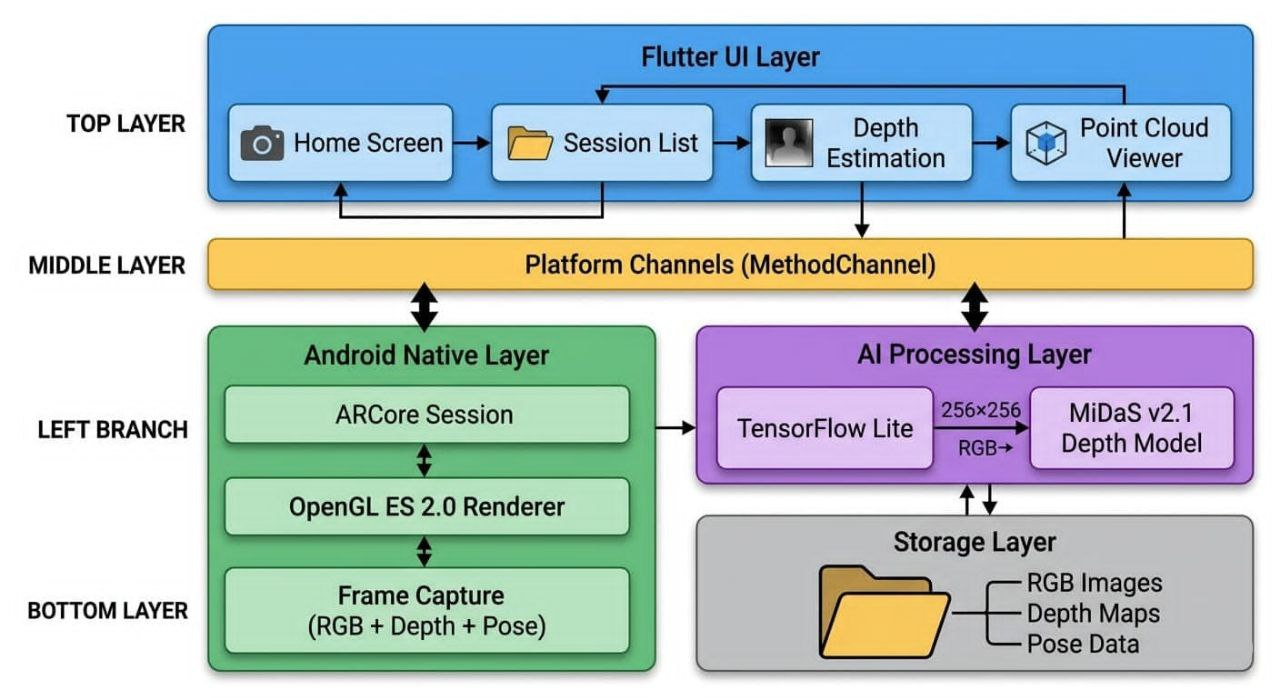
\includegraphics[width=0.85\textwidth]{architecture.png}
\end{center}

Pipeline of the proposed system:

\begin{center}
Image Capture $\rightarrow$ Depth Estimation $\rightarrow$ Point Cloud Generation $\rightarrow$ 3D Visualization
\end{center}
\end{frame}

\section{Implementation Details}

\begin{frame}{Hardware Configuration}
\begin{itemize}
\item ARM-based Android smartphone
\item Minimum 4GB RAM
\item Mobile camera for image capture
\item Development system with GPU support for model conversion
\end{itemize}
\end{frame}

\begin{frame}{Software Configuration}
\begin{itemize}
\item Flutter (Dart) for mobile application development
\item TensorFlow Lite for on-device machine learning inference
\item ARCore for camera pose estimation and depth capture
\item OpenCV for image processing tasks
\item Python for model preparation and conversion
\end{itemize}
\end{frame}

\section{Benchmark Criteria and Methodology}

\begin{frame}{Benchmark Objective}
    \textbf{Primary Goal:} Evaluate and compare the computational throughput and inference latency of a depth estimation model across distinct hardware architectures.
    \vspace{0.5cm}
    \begin{itemize}
        \item \textbf{Target Model:} MiDaS v2.1 Small.
        \item \textbf{Metrics Evaluated:} Inference latency, throughput (FPS), and resource utilization.
        \item \textbf{Hardware Compared:} Edge mobile deployment vs. Standard host baseline.
    \end{itemize}
\end{frame}

\begin{frame}{Evaluated Workload \& Environments}
    \textbf{Workload Constraints}
    \begin{itemize}
        \item \textbf{Input Shape:} $[1, 3, 256, 256]$ (RGB images).
        \item \textbf{Model Format:} TensorFlow Lite \texttt{.tflite} (FlatBuffer).
    \end{itemize}
    \vspace{0.5cm}
    \textbf{Hardware Environments}
    \begin{itemize}
        \item \textbf{Edge Environment:} ARM64 Android device (Target Deployment).
        \item \textbf{Host Environment:} x86\_64 Windows system (Computational Baseline).
    \end{itemize}
\end{frame}

\begin{frame}{Execution Methodology}
    To eliminate high-level software bottlenecks, the evaluation is strictly controlled:
    \vspace{0.5cm}
    \begin{itemize}
        \item \textbf{Native Execution:} Benchmarks run directly via official LiteRT \texttt{benchmark\_model} C++ binaries.
        \item \textbf{Thread Standardization:} CPU thread count is explicitly locked to 4 threads across both devices.
        \item \textbf{Hardware Delegation:} Both environments leverage the XNNPack CPU delegate for optimized vector math instructions.
        \item \textbf{Warmup Phase:} Mandatory warmup iterations are executed before profiling to prevent "cold start" CPU throttling.
    \end{itemize}
\end{frame}

\begin{frame}{Primary Performance Metrics}
    Data is aggregated over 50 sustained iterations to ensure statistical significance:
    \vspace{0.5cm}
    \begin{itemize}
        \item \textbf{Initialization Time (ms):} Time required to load the graph and initialize runtime delegates.
        \item \textbf{Average Inference Latency (ms):} Mean time to execute a single forward pass.
        \item \textbf{Throughput (FPS):} Maximum theoretical frames per second based on average latency.
        \item \textbf{Memory Footprint (MB):} Approximate RAM allocated during active inference.
    \end{itemize}
\end{frame}


\begin{frame}{Model Parameters}
\begin{itemize}
\item Depth Estimation Model: MiDaS Small
\item Input Image Size: 256 $\times$ 256
\item Model Format: TensorFlow Lite (.tflite)
\item Output: Relative depth map
\item Optimization: Quantization and lightweight inference for mobile devices
\end{itemize}
\end{frame}

\begin{frame}{Performance Analysis}
\begin{itemize}
\item Average depth estimation time: 0.5-1 second per frame
\item Point cloud generation: Real-time processing
\item Memory usage optimized for mobile devices
\item CPU-based rendering reduces GPU dependency
\end{itemize}
\end{frame}

\begin{frame}{Result of Benchmark}
    \textbf{1. ARM64 Mobile Device (Nothing Phone 2a - MediaTek Dimensity 7200 Pro)}
    \begin{center}
    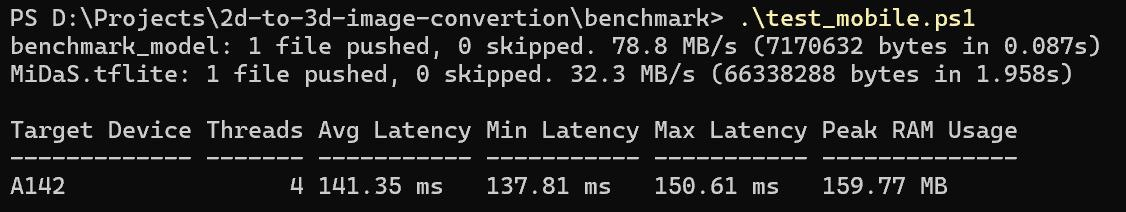
\includegraphics[width=0.96\textwidth]{benchmark_mob.jpg}
    \end{center}
    
    \vspace{0.3cm}
    
    \textbf{2. x86\_64 Desktop (Intel Core Ultra 7 255H)}
    \begin{center}
    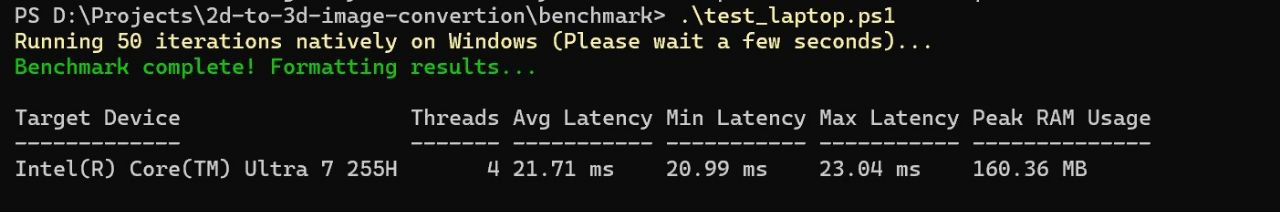
\includegraphics[width=0.96\textwidth]{benchmark_lap.jpg}
    \end{center}
\end{frame}

\begin{frame}{Result of Benchmark}
    \vspace{0.3cm}
    \textbf{Key Observations:}
    \begin{itemize}
        \item \textbf{Architectural Throughput Gap:} The x86\_64 computational host processes frames approximately 6.5$\times$ faster than the ARM64 edge device.
        \item \textbf{Edge Viability:} Achieving sub-150ms latency entirely on a mobile CPU demonstrates that the model is highly viable for near-real-time edge deployment.
        \item \textbf{Memory Determinism:} Peak RAM allocation remains strictly consistent ($\sim$160 MB) despite crossing distinct OS boundaries and hardware instruction sets.
    \end{itemize}
    
\end{frame}

\section{Future Prospects}

\begin{frame}{Future Prospects}
\begin{itemize}
\item Improve depth estimation accuracy using advanced models.
\item Extend the system for real-time video-based reconstruction.
\item Add mesh reconstruction and texture mapping.
\item Integrate with augmented reality and robotics applications.
\end{itemize}
\end{frame}

% --------------------------------------
\section{Conclusion}

\begin{frame}{Conclusion}
\textbf{The proposed Offline 2D-to-3D Reconstruction System} addresses the limitations of existing solutions by:

\begin{itemize}
    \item Achieving \textbf{fully offline} 3D reconstruction without reliance on cloud servers.
    \item Combining \textbf{lightweight neural networks} for depth estimation with \textbf{geometric processing} for depth fusion and mesh generation.
    \item Enabling \textbf{real-time processing} directly on \textbf{resource-constrained ARM-based mobile devices}.
\end{itemize}

\medskip
This framework provides an \textbf{efficient, portable, and privacy-preserving} alternative, contributing to the \textbf{democratization of 3D reconstruction} for mobile and embedded systems.
\end{frame}

% --------------------------------------
\section{Future Work}

\begin{frame}{Future Work}
The proposed system can be further enhanced in the following directions:

\medskip
\begin{itemize}
\item Integration of \textbf{advanced depth estimation models} to improve reconstruction accuracy and robustness.
\item Extension to \textbf{real-time video-based 3D reconstruction} for continuous scene capture.
\item Optimization for \textbf{wider deployment on mobile and embedded platforms}.
\item Incorporation of \textbf{texture mapping and color refinement} for more realistic 3D models.
\item Exploration of \textbf{augmented reality (AR) and robotics applications} using the reconstructed 3D environment.
\end{itemize}
\end{frame}

% --------------------------------------
\section{References}
\begin{frame}[allowframebreaks]{References}
\scriptsize
\begin{thebibliography}{9}
\bibitem{tochilkin2024}
D. Tochilkin et al. (2024).
\newblock TripoSR: Fast 3D Object Reconstruction from a Single Image.
\newblock \textit{arXiv (CVPR-style research)}.

\bibitem{yang2020}
X. Yang et al. (2020).
\newblock Mobile3DRecon: Real-time Monocular 3D Reconstruction on a Mobile Phone.
\newblock \textit{IEEE TVCG}.

\bibitem{papa2024}
L. Papa et al. (2024).
\newblock METER: A Mobile Vision Transformer Architecture for Monocular Depth Estimation.
\newblock \textit{IEEE Journal / arXiv}.

\bibitem{li2022}
Z. Li et al. (2022).
\newblock LiteDepth: Digging into Fast and Accurate Depth Estimation on Mobile Devices.
\newblock \textit{ECCV / MAI Challenge}.

\bibitem{luo2024}
H. Luo et al. (2024).
\newblock Large-Scale 3D Reconstruction from Multi-View Imagery: A Comprehensive Review.
\newblock \textit{Remote Sensing (MDPI)}.

\bibitem{smith2023}
A. Smith et al. (2023).
\newblock 3D Reconstruction Using Deep Learning: A Survey.
\newblock \textit{IEEE Transactions on Pattern Analysis and Machine Intelligence}.


\bibitem{johnson2022}
B. Johnson et al. (2022).
\newblock Real-Time 3D Object Reconstruction and Distance Estimation from 2D Images.
\newblock \textit{International Journal of Computer Vision}.

\bibitem{lee2023}
C. Lee et al. (2023).
\newblock ZoeDepth: Zero-shot Transfer by Combining Relative and Metric Depth.
\newblock \textit{arXiv}.
\end{thebibliography}
\end{frame}

% --------------------------------------
\begin{frame}
\begin{center}
    \Huge{Thank You!}
\end{center}
\end{frame}

\end{document}